\documentclass[tikz,border=4pt]{standalone}
\usepackage{amsmath,bm}
\usetikzlibrary{arrows.meta,calc,decorations.markings}
\begin{document}
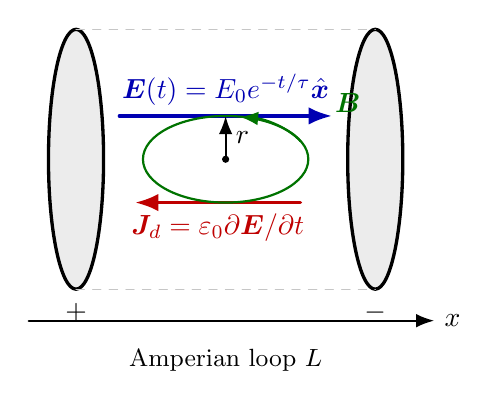
\begin{tikzpicture}[scale=1.0,>=Latex,line cap=round,line join=round]
  \coordinate (A) at (0,0);
  \coordinate (B) at (3.8,0);

  \draw[fill=gray!15,draw=black,very thick] (A) ellipse (0.35 and 1.65);
  \draw[fill=gray!15,draw=black,very thick] (B) ellipse (0.35 and 1.65);
  \draw[gray!45,dashed] (0,-1.65) -- (3.8,-1.65);
  \draw[gray!45,dashed] (0,1.65) -- (3.8,1.65);

  \draw[->,very thick,blue!70!black] (0.55,0.55) -- (3.25,0.55)
    node[midway,above] {$\bm E(t)=E_0e^{-t/\tau}\hat{\bm x}$};
  \draw[->,very thick,red!75!black] (2.85,-0.55) -- (0.75,-0.55)
    node[midway,below] {$\bm J_d=\varepsilon_0\partial\bm E/\partial t$};

  \draw[->,thick] (-0.6,-2.05) -- (4.55,-2.05) node[right] {$x$};
  \draw[->,thick] (1.9,0) -- (1.9,0.55) node[midway,right] {$r$};
  \fill (1.9,0) circle (1.3pt);

  \draw[thick,green!45!black] (1.9,0) ellipse (1.05 and 0.55);
  \draw[->,green!45!black,thick] (2.85,0.23) arc[start angle=25,end angle=80,x radius=1.05,y radius=0.55];
  \node[green!45!black] at (3.45,0.72) {$\bm B$};

  \node at (0,-1.95) {$+$};
  \node at (3.8,-1.95) {$-$};
  \node at (1.9,-2.55) {\small Amperian loop $L$};
\end{tikzpicture}
\end{document}
